\documentclass[addpoints]{exam}
\usepackage[utf8]{inputenc}
\usepackage{amsmath}
\usepackage{mathtools}
\usepackage{tikz}
\usepackage{pgfplots}
\usetikzlibrary{datavisualization}
\usetikzlibrary{datavisualization.formats.functions}
\usepackage{relsize}
\usepackage{dirtytalk}
\usepackage{graphicx}
\graphicspath{ {./drift/} }
\DeclarePairedDelimiter{\ceil}{\lceil}{\rceil}
\usepackage{geometry}
\usepackage{draftwatermark}
\SetWatermarkFontSize{2cm}
\SetWatermarkText{Mathematics-1998}
\usepackage[banglamainfont=Kalpurush, 
            banglattfont=Siyam Rupali
           ]{latexbangla}
        
\begin{document}
\begin{LARGE}
\begin{center}
গণিত (Mathematics - 1998)
\end{center}
\end{LARGE}
\begin{questions}

     \question  $ \dfrac{2x}{(x-1)(x^2 +1)} \equiv \dfrac{A}{x-1} + \dfrac{Bx+1}{x^2 +1} $  অভেদে (A,B) এর মান হবে (In the identity (A, B) equals)

\begin{oneparchoices}
\choice $ (-1,-1) $
\choice $ (-1, 1) $
\choice $ (1,-1) $
\choice  $ (1,1) $
\end{oneparchoices}

\question একটি সরলরেখা $(3,5)$ বিন্দু দিয়ে যায় এবং অক্ষদ্বয় থেকে বিপরীত চিহ্ন বিশিষ্ট ছেদ করে। সরলরেখাটির সমীকরণ কি? (What is the equation of the straight line passing through a point $(3,5)$ and intersect a part of same magnitude but opposite sign from the axis? ) 

\begin{oneparchoices}
\choice $ x-y+2=0 $
\choice $ x-2y+7=0 $
\choice $ x-y-8=0 $
\choice $ 2x-2y+1=0 $
\end{oneparchoices}


\question  $ \tan (-15^{\circ}) $ এর মান- (The value of  $ \tan (-15^{\circ}) $ is)

\begin{oneparchoices}
\choice  $ -\dfrac{1}{2\sqrt{3}} $
\choice  $ \sqrt{5} $
\choice  $ \sqrt{3} - 2 $
\choice  $ \sqrt{2}- 3 $
\end{oneparchoices}

\question যদি $ \mathlarger{\int}\sin 5x\cos x\, dx =f(x) + c $  যেখানে একটি ধ্রুবক তবে $ f(x)+c = ?$ (If $ \mathlarger{\int}\sin 5x\cos x\, dx =f(x) + c $ where $ c $ is a constant, then $ f(x)+c =? $ )


\begin{oneparchoices}
\choice  $ \dfrac{1}{6}\cos^{6} x $
\choice  $ \dfrac{1}{6}\sin^{6}x $
\choice  $ \dfrac{1}{6}\cos^{5}x\sin x $
\choice  $ -\dfrac{1}{6}\cos^{6}x $
\end{oneparchoices}


\question একটি ট্রেন স্টেশন $ S  $ এ স্থিতাবস্থা থেকে শুরু করে ধ্রুব ত্বরণ সহকারে চলতে থাকে। যাত্রা শুরুর 15 সেকেন্ড পরে ট্রেনটি সিগনাল বক্স অতিক্রম করে এবং তখন তার দ্রুতি । ট্রেনটিকে একটি কণা বিবেচনা করে স্টেশন এবং সিগনাল বক্স এর দুরত্ব আসন্ন মিটারে হিসাব করা হল। এই দুরত্ব কত?

\begin{oneparchoices}
\choice 330 m
\choice 300 m
\choice 185 m
\choice 165 m
\end{oneparchoices}

\question $ 3x^{2}+2x+1=0 $ সমীকরণের মূলদ্বয়ের বর্গের সমষ্টি কত?

\begin{oneparchoices}
\choice $ -\dfrac{2}{3} $
\choice  $ \dfrac{2}{9} $
\choice $ \dfrac{2}{3} $
\choice $ -\dfrac{2}{9} $  
\end{oneparchoices}

\question  $ 3x^{2}+3y^{2}+6x-12y-15=0  $ সমীকরণ দ্বারা বর্ণিত বৃত্তের কেন্দ্র কি?

\begin{oneparchoices}
\choice $ (-3,6) $
\choice $ (1,-2) $
\choice $ (-1,2) $
\choice $ (6,-12) $
\end{oneparchoices}

\question $ \dfrac{2\tan Q}{1+\tan^{2} Q} =?  $  

\begin{oneparchoices}
\choice $ \tan 2Q $
\choice $ 2\sin Q\cos Q $
\choice $ 2\cos^{2}\dfrac{Q}{2} $
\choice $ \cos 2Q $
\end{oneparchoices}

\question $ x=\cos\theta,\, y= \cos\theta +\sin\theta $  হলে $ \dfrac{dy}{dx} = ? $

\begin{oneparchoices}
\choice $ 1-\cot\theta $
\choice $ 1-\tan\theta $
\choice $ 1+\cot\theta $
\choice $ \cot\theta - 1 $
\end{oneparchoices}


\question  যদি A বিন্দুতে একটি কণা পাশের চিত্রের প্রদর্শিত ভাবে কার্যরত পরিমাপের বল দ্বারা স্থিতাবস্থায় থাকে, তবে T কত?

\begin{oneparchoices}
\choice  $ w-P $
\choice  $ P-w $ 
\choice  $ P+\sqrt{2} w$
\choice  $ \dfrac{\sqrt{2}P}{w} $ 
\end{oneparchoices}


\question  নির্ণায়ক $ \begin{vmatrix}
10 & 11 & 12\\
20 & 21 & 24\\
10 & 10 & 10
\end{vmatrix} $ এর মান কত?

\begin{oneparchoices}
\choice $ 10 $
\choice $ 20 $
\choice $ 1 $
\choice $ 0 $
\end{oneparchoices}

\question $ 3(x-1)^{2}+4y^{2}=12 $ সমীকরণ কি বর্ণনা করে?

\begin{oneparchoices}
\choice বৃত্ত যার কেন্দ্র $(1,0)$ \\
\hspace*{-.3cm}\choice পরাবৃত্ত যার শীর্ষ $(1,0)$\\ 
\hspace*{-.3cm}\choice উপবৃত্ত যার একটি ফোকাস $(1,0)$\\
\hspace*{-.3cm}\choice উপবৃত্ত যার একটি ফোকাস $(0,0)$
\end{oneparchoices}

\question (The general solution of the following equation is) $ \cos\theta = \dfrac{1}{2} $ সমীকরনের সাধারণ সমাধান- (এখানে $ n $ একটি পূর্ন সংখ্যা নির্দেশ করে) (Here $ n $ is an integer.)

\begin{oneparchoices}
\choice $ \theta = 2n\pi \pm\dfrac{\pi}{6} $
\choice $ \theta = n\pi +\dfrac{\pi}{3} $
\choice $ \theta = 2n\pi +\dfrac{\pi}{3} $
\choice $ \theta = 2n\pi \pm \dfrac{\pi}{3} $
\end{oneparchoices}

\question  $ \dfrac{d}{dx} (\log_{3}2x^{3}) =? $


\begin{oneparchoices}
\choice $ \dfrac{1}{3x} $ 
\choice $ \dfrac{x}{3} $
\choice $ 2x^{-\frac{1}{3}} $
\choice $ \dfrac{2}{3x^{\frac{2}{3}}} $
\end{oneparchoices}

\question একটি কণা আনুভূমিক তলের সাথে $ \theta $ কোণে $ a $ বেগ সহকারে প্রক্ষেপ করা হল। আনুভূমিক তল থেকে কনাটি সর্বাধিক উচ্চতা কত হবে? 

\begin{oneparchoices}
\choice $\dfrac{a^{2}\sin^{2}\theta}{2g} $
\choice $\dfrac{a^{2}\sin^{2}2\theta}{g} $
\choice $\dfrac{a^{2}\sin\theta}{2g} $
\choice $\dfrac{a^{2}\sin 2\theta}{g} $
\end{oneparchoices}


\question $ (1+px)^{5} $ এর বিস্তৃতিতে $ x $ এর সহগ এবং $ \Big(9+\dfrac{x}{3}\Big)^{6} $ এর বিস্তৃতিতে $ x^{8} $ এর সহগ সমান হলে $ p $ এর মান কত?

\begin{oneparchoices}
\choice $ 1 $
\choice $ \dfrac{1}{3} $
\choice $ 3 $
\choice $ 9 $
\end{oneparchoices}

\question  $ 4x-3y=9 $ সরলরেখা থেকে $ (-2,1) $ বিন্দুর দুরত্ব কত?

\begin{oneparchoices}
\choice $ 9 $
\choice $ 4 $
\choice $ -8 $
\choice $ 20 $
\end{oneparchoices}

\question যদি $ \dfrac{\pi}{2}<\theta<\pi $ এবং $ \sin\theta =\dfrac{5}{12} $ হয় তবে, $ \dfrac{\tan\theta + \sec (\theta)}{\cot\theta + \csc (-\theta)} $ এর মান কত?


\begin{oneparchoices}
\choice $ \dfrac{3}{10} $
\choice $ -\dfrac{5}{3} $
\choice $ \dfrac{3}{5} $
\choice $ \dfrac{1}{2} $
\end{oneparchoices}

\question $ \mathlarger{\int_{0}^{1}}\dfrac{x}{2-x^{2}}dx $ এর মান কত?

\begin{oneparchoices}
\choice $ 1 $ 
\choice $ \dfrac{1}{2}\log_{e} 2 $ 
\choice $ 2 $
\choice $ \log_{e} 2 $
\end{oneparchoices}

\question একটি কণা আনুভূমিক তল থেকে 78.4 মি উচু কোন স্থান থেকে আনুভূমিক ভাবে প্রক্ষেপ করা হয় এবং t সময়ে পরে তা ঐ আনুভূমিক তলে পতিত হয়। g =9.8 মি/সে$ ^{2} $ ধরা হলে t কত?

\begin{oneparchoices}
\choice  9.8 sec
\choice  7.8 sec
\choice 3 sec
\choice 4 sec
\end{oneparchoices}

\question $ \dfrac{1}{2}(e^{x}-e^{-x}) $ এর ধারা বিস্তৃতি কি?


\begin{oneparchoices}
\choice  $ 1+\dfrac{x^{2}}{3!}+\dfrac{x^{2}}{3!}+\cdots\cdots $
\choice  $ 1-\dfrac{x^{2}}{3!}+\dfrac{x^{2}}{3!}-\cdots\cdots $\\
\hspace*{-.3cm}\choice  $ x+\dfrac{x^{2}}{3!}+\dfrac{x^{2}}{3!}+\cdots\cdots $
\choice  $ x-\dfrac{x^{2}}{3!}+\dfrac{x^{2}}{3!}+\cdots\cdots $
\end{oneparchoices}

\question  নিচের কোনটি $y=(x+1)^2$ এর লেখচিত্র? 

\begin{oneparchoices}
 \choice 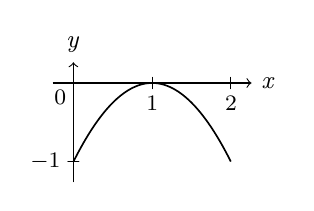
\begin{tikzpicture}
\datavisualization [school book axes,
                    visualize as smooth line,
                    y axis={label},
                    x axis={label} ]

data [format=function] {
      var x : interval [0:2] samples 150;
      func y =  2*\value x -  \value x*\value x - 1 ;
      };
\end{tikzpicture}
 \choice 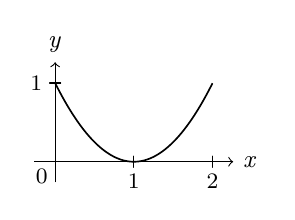
\begin{tikzpicture}
\datavisualization [school book axes,
                    visualize as smooth line,
                    y axis={label},
                    x axis={label} ]

data [format=function] {
      var x : interval [0:2] samples 150;
      func y =   \value x*\value x-2*\value x + 1 ;
      };
\end{tikzpicture}
\choice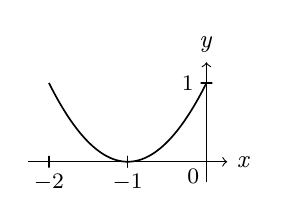
\begin{tikzpicture}
\datavisualization [school book axes,
                    visualize as smooth line,
                    y axis={label},
                    x axis={label} ]

data [format=function] {
      var x : interval [-2:0] samples 150;
      func y =   \value x*\value x+2*\value x + 1 ;
      };
\end{tikzpicture}
 \choice 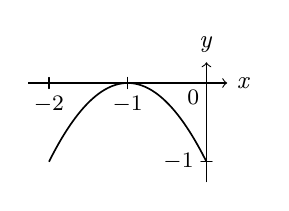
\begin{tikzpicture}
\datavisualization [school book axes,
                    visualize as smooth line,
                    y axis={label},
                    x axis={label} ]

data [format=function] {
      var x : interval [-2:0] samples 150;
      func y =   -\value x*\value x-2*\value x - 1 ;
      };
\end{tikzpicture}
 
\end{oneparchoices}

\question $ x $ এর কোন ধনাত্নক মানের জন্য $ y=x+\dfrac{1}{x} $ এর ঢাল শূণ্য?

\begin{oneparchoices}
\choice  $ 2 $
\choice  $ 1 $
\choice  $ \sqrt{2} $
\choice  $ \dfrac{1}{2} $
\end{oneparchoices}

\question $ \mathlarger{\int_{0}^{1}}\dfrac{\sin^{-1}x}{\sqrt{1-x^{2}}}dx  $ এর মান কত?

\begin{oneparchoices}
\choice $ \dfrac{\pi}{4} $
\choice $ \dfrac{1}{2} $
\choice $ \dfrac{\pi^{2}}{8} $
\choice  $ \pi $
\end{oneparchoices}

 \question যদি TIME শব্দটির অক্ষরগুলোর পূনর্বিন্যাস করা হয় তবে কতগুলো বিন্যাস স্বরবর্ণ দ্বারা শুরু হয়?

\begin{oneparchoices}
\choice 6
\choice 24
\choice 32
\choice 12
\end{oneparchoices}

\end{questions}

\end{document}